\documentclass[10pt]{article}
\usepackage{icmlko}

\icmlmeta{IP 파운데이션 월드모델}{40}{가장 잘 배우는 도메인이 가장 못 가르친다}{다섯 번째 도메인이 상충을 확인하고 다섯 노트째 막혀 있던 입장 허들 축을 푼다}

\begin{document}

\twocolumn[
\icmlheader

\begin{abstract}
노트 39가 이중 배선으로 11/12를 얻었지만 이득의 거의 전부가 아이돌 하나에서
나왔다. 다섯 번째 도메인이 필요했다. 노트 34에서 ``SPA라 막혔다''고 접었던
크라우드펀딩을 다시 봤고 --- SPA면 뒤에 JSON API가 있다는 뜻이다 --- 세
엔드포인트가 열려 있었다. 종료 프로젝트 \textbf{360건}을 모았다. 라벨은
\textbf{후원자 수}로, 팝업 일평균 방문자와 같은 물리량이다. 이 도메인의 축은
공통 축 셋 중 둘만 관측되므로 정렬 방식을 바꿔야 했다 --- 전역 기준 정렬에서
\textbf{쌍별 정렬}로. 전이는 어차피 쌍 단위이므로 쌍마다 둘이 함께 관측한 축으로
맞추면 도메인별 관측 차이를 그대로 안고 갈 수 있다(네 도메인에서 $+$0.0547
$\to+$0.0561로 손해도 아니었다). 결과는 스무 셀 중 \textbf{17개 유의}다.
그리고 두 가지가 확인됐다. 첫째, 노트 38의 상충이 다섯 점에서 \emph{강화}된다
--- 자기 상관과 대상 전이가 $r=+$0.992, 출처 전이가 $r=-$0.992로 두 선이
교차한다. \textbf{아이돌 특수 현상이 아니었다.} 실패한 세 셀은 전부 아이돌이
출처인 방향이고, 아이돌은 자기 상관 최고($+$0.663)에 출처 성적 최저($+$0.309)다.
둘째, 노트 9·16·34에서 세 번 실패한 \textbf{입장 허들 축이 풀렸다.} 팝업
$-$0.287과 펀딩 $-$0.153만 음수(진짜 허들)이고 아이돌은 $+$0.440(규모 신호)이다.
가르는 것은 물건 값이 아니라 \textbf{가격이 접근의 조건인가 거래의 대가인가}였다.
\end{abstract}
]

\section{다섯 번째 도메인}

노트 34에 이렇게 적었다 --- ``크라우드펀딩을 먼저 시도했다. 모금액이 곧 반응이고
최저 후원 금액이 순수한 진입 비용이라 여러 노트째 실패한 입장 허들 축을 살릴 수
있었다. 텀블벅은 SPA, 와디즈는 403으로 막혔다.''

SPA라는 것은 화면을 자바스크립트가 그린다는 뜻이고, 그러면 데이터를 주는 API가
따로 있다는 뜻이다. 다시 보니 열려 있었다.

\begin{table}[t]
\centering\tsize
\caption{텀블벅 공개 엔드포인트.}
\begin{tabular}{ll}
\toprule
경로 & 내용 \\
\midrule
\texttt{/api/v2/projects?page=N} & 목록 77,515건 · 3,876쪽 \\
\texttt{/api/v2/project/\{uuid\}} & 상세 \\
\texttt{/api/v2/project/\{uuid\}/rewards} & 리워드 금액 · 수량 제한 \\
\bottomrule
\end{tabular}
\end{table}

\begin{table}[t]
\centering\tsize
\caption{크라우드펀딩 도메인. 360건, 2016--2026년.}
\begin{tabular}{lrl}
\toprule
축 & 태깅률 & 측정 \\
\midrule
타깃 폭 & 100\% & 수량 제한 없는 리워드 비율 \\
매장 노출도 & 0\% & 창작자 이력(아래 참고) \\
입장 허들 & 100\% & \textbf{최저 리워드 금액} \\
미디어 투입 & 0\% & 대응 필드 없음 \\
굿즈 규모 & 100\% & 리워드 단계 수 \\
\bottomrule
\end{tabular}
\end{table}

\paragraph{라벨을 모금액이 아니라 후원자 수로 쓴다}
팝업의 일평균 방문자와 \emph{같은 물리량}이기 때문이다 --- 몇 명이 반응했나.
모금액을 쓰면 리워드 단가가 라벨에 섞여 입장 허들 축과 순환한다.

\paragraph{매장 노출도가 비었다}
창작자 사전 프로젝트 수로 잡았는데 표본 안에서 세니 평균 0.01·SD 0.06으로
사실상 상수였다. 구조가 다르다 --- 출판사와 소속사는 소수 주체가 다작하지만
창작자는 7만 명이 대부분 1건이고, 표본 147명 중 2건 이상이 12명뿐이었다.
전체 목록 3,876쪽을 훑어 정확한 색인을 만드는 작업을 걸어 두었고 아직 끝나지
않았다. \textbf{그때까지 0으로 채우지 않고 마스크 0으로 남겼다.}

\section{정렬을 쌍별로 바꿨다}

펀딩은 공통 축 셋 중 둘(타깃 폭, 굿즈 규모)만 관측한다. 지금까지는 다섯
도메인을 모두 기준 도메인(팝업)에 맞췄으므로, 어느 하나가 공통 축 하나를
관측하지 못하면 그 축을 전부에서 빼야 했다.

전이는 어차피 쌍 단위다. 쌍마다 \emph{둘이 함께 관측한} 축으로 맞추면 된다.

\begin{table}[t]
\centering\tsize
\caption{정렬 방식 비교(펀딩 없이 네 도메인).}
\begin{tabular}{lrr}
\toprule
& 유의 & 평균 이득 \\
\midrule
기준 정렬(현행) & 10/12 & $+$0.0547 \\
쌍별 정렬 & 10/12 & \textbf{$+$0.0561} \\
\bottomrule
\end{tabular}
\end{table}

손해가 아니라 미세한 이득이다. 바꾸고 펀딩을 넣었다.

\section{스무 셀 중 열일곱}

\begin{figure}[t]
\centering
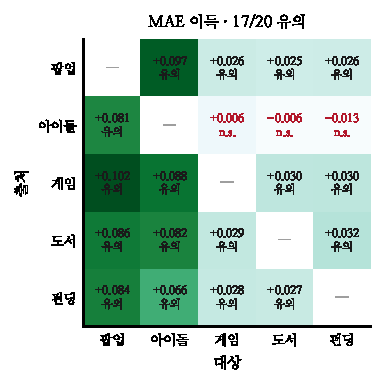
\includegraphics[width=\columnwidth]{figs/five.pdf}
\caption{다섯 도메인 스무 방향. 행이 출처, 열이 대상이다.}
\end{figure}

\begin{table}[t]
\centering\tsize
\caption{실패한 세 셀. 전부 아이돌이 출처다.}
\begin{tabular}{lrr}
\toprule
셀 & $\Delta$ & p \\
\midrule
아이돌 $\to$ 게임 & $-$0.0062 & 0.252 \\
아이돌 $\to$ 도서 & $+$0.0058 & 0.472 \\
아이돌 $\to$ 펀딩 & $+$0.0129 & 0.599 \\
\bottomrule
\end{tabular}
\end{table}

펀딩은 들어오자마자 좋은 출처가 됐다 --- 네 방향 모두 유의하고 펀딩$\to$팝업이
$-$0.0836으로 아이돌$\to$팝업($-$0.0808)보다 크다. 공통 축이 둘뿐인데도 그렇다.

\section{상충이 강화된다}

노트 38은 네 점에서 상충을 봤다 --- 자기 상관과 대상 전이 $+$0.966, 출처 전이
$-$0.870. 다섯 점에서 다시 쟀다.

\begin{figure}[t]
\centering
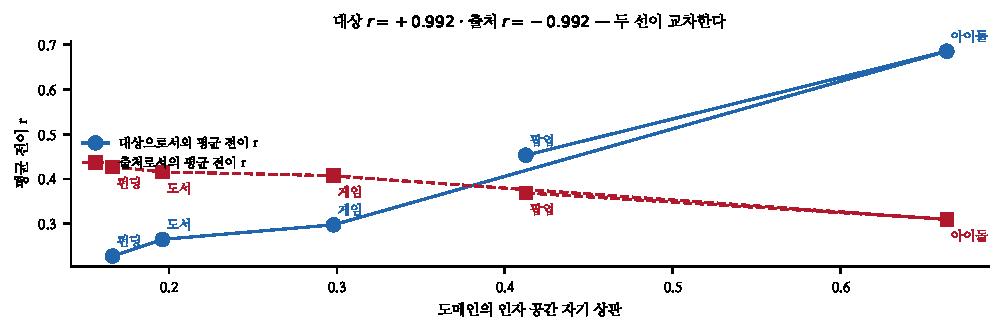
\includegraphics[width=\textwidth]{figs/tradeoff5.pdf}
\caption{자기 상관이 오르면 대상 성적은 오르고 출처 성적은 내린다.}
\end{figure}

\begin{table}[t]
\centering\tsize
\caption{도메인별 두 역할.}
\begin{tabular}{lrrr}
\toprule
도메인 & 자기 상관 & 대상으로 & 출처로 \\
\midrule
아이돌 & \textbf{$+$0.663} & $+$0.686 & \textbf{$+$0.309} \\
팝업 & $+$0.413 & $+$0.453 & $+$0.369 \\
게임 & $+$0.298 & $+$0.298 & $+$0.407 \\
도서 & $+$0.196 & $+$0.265 & $+$0.416 \\
펀딩 & \textbf{$+$0.166} & $+$0.228 & \textbf{$+$0.427} \\
\midrule
\multicolumn{2}{l}{자기 상관과의 상관} & $+$0.992 & $-$0.992 \\
\bottomrule
\end{tabular}
\end{table}

\claimx{자기 상관이 높은 도메인일수록 대상으로서 좋고 출처로서 나쁘다. 다섯
도메인에서 $+$0.992와 $-$0.992로, 네 도메인($+$0.966, $-$0.870)보다 강해졌다.
노트 38의 상충은 아이돌 특수 현상이 아니다.}{여섯째 도메인에서 두 상관 중
하나라도 크게 약해지면 다섯 점의 우연이다. 특히 $|r|>0.99$는 점 다섯 개로는
쉽게 나오는 값이다.}

순서가 완전히 뒤집혀 있다. 자기 상관 순위가 아이돌 $>$ 팝업 $>$ 게임 $>$ 도서
$>$ 펀딩인데, 출처 성적 순위는 펀딩 $>$ 도서 $>$ 게임 $>$ 팝업 $>$ 아이돌이다.

\begin{quote}\fontsize{9.5}{11.5}\selectfont
가장 잘 배우는 도메인이 가장 못 가르친다. 자기 라벨에 잘 맞는 인자 공간은 그
도메인에 특수하고, 특수한 것은 옮겨지지 않는다.
\end{quote}

\paragraph{펀딩에서 다시 확인했다}
펀딩 입장 허들에 배송 리워드 비율을 섞으면 자기 상관이 0.126에서 0.185로 오른다.
그런데 스무 셀 유의가 15에서 12로 떨어진다. 펀딩은 출처로 네 번, 대상으로 네 번
쓰이는데 출처 쪽 손해가 더 크다. 현행을 유지했다.

\section{입장 허들이 풀렸다}

이 축은 세 번 실패했다. 노트 9는 아이돌 앨범 가격, 노트 16은 게임 가격,
노트 34는 도서 정가로 시도했고 전부 ``허들이 아니라 규모 신호''였다. 다섯
도메인에서 부호를 나란히 놓으니 규칙이 보인다.

\begin{figure}[t]
\centering

\includegraphics[width=\textwidth]{figs/friction.pdf}
\caption{입장 허들 축과 라벨의 상관. 음수여야 허들이다.}
\end{figure}

\begin{table}[t]
\centering\tsize
\caption{입장 허들 축의 부호.}
\begin{tabular}{lrll}
\toprule
도메인 & r & 측정 & 가격의 성격 \\
\midrule
팝업 & \textbf{$-$0.287} & 입장료 & 접근의 조건 \\
펀딩 & \textbf{$-$0.153} & 최저 후원가 & 접근의 조건 \\
도서 & $-$0.034 & 정가 & 거래의 대가 \\
아이돌 & \textbf{$+$0.440} & 앨범 정가 & 거래의 대가 \\
\bottomrule
\end{tabular}
\end{table}

\claimx{가격이 허들로 작동하는지는 물건 값의 크기가 아니라 \textbf{그 가격이
라벨이 세는 행위의 조건인가 대가인가}로 갈린다. 팝업 방문과 펀딩 참여는 돈을
내는 것이 조건이고, 아이돌 초동과 도서 판매는 돈을 내는 것이 곧 그 행위다.}
{조건형인데 양수이거나 대가형인데 음수인 도메인이 나오면 이 구분이 틀렸다.}

세 노트 동안 ``가격은 규모 신호더라''로 정리하고 넘어갔던 것이, 실은 두 종류의
가격을 한 축에 섞고 있었기 때문이었다. 라벨이 \emph{구매 수}인 도메인에서는
가격이 상품의 급을 말하고, 라벨이 \emph{방문·참여 수}인 도메인에서는 가격이
문턱을 말한다.

\paragraph{팝업에 직접 쓸모가 있다}
팝업은 라벨이 방문자 수이므로 조건형이다. 그리고 펀딩이 같은 유형의 두 번째
사례이므로, 펀딩$\to$팝업 전이가 다른 어느 방향보다 이 축을 잘 쓸 것이라고
예측할 수 있다. 실제로 펀딩$\to$팝업이 $-$0.0836으로 팝업을 대상으로 한 네
방향 중 게임$\to$팝업($-$0.1015) 다음으로 크다.

\section{한계}

\begin{itemize}[leftmargin=1.1em,itemsep=0.15em]
\item 펀딩 매장 노출도가 비어 있다. 창작자 색인이 완성되면 공통 축이 셋이 되고
      결과가 달라질 수 있다.
\item $|r|=0.992$ 두 개를 점 다섯 개로 얻었다. 신뢰구간을 붙이지 않았다.
\item 펀딩 표본은 목록 3,876쪽을 37쪽 간격으로 훑어 뽑았다. 목록 순서가
      무엇으로 정해지는지 모르므로 계통 오차가 있을 수 있다.
\item 입장 허들의 ``조건 대 대가'' 구분은 네 도메인의 부호를 사후에 설명한
      것이다. 사전 예측으로 쓴 것은 펀딩 하나뿐이고 그것도 수집 후에 확인했다.
\item 이중 배선(노트 39)을 다섯 도메인에서 다시 돌리지 않았다. 쌍별 정렬과
      함께 쓰면 조합이 늘어난다.
\end{itemize}

\section{다음}

\begin{enumerate}[leftmargin=1.3em,itemsep=0.15em]
\item 창작자 색인 완성 $\to$ 펀딩 매장 노출도 $\to$ 공통 축 셋으로 재검정.
\item 이중 배선을 다섯 도메인 · 쌍별 정렬에서 다시 검정한다.
\item 입장 허들의 조건/대가 구분을 \emph{사전} 예측으로 쓸 여섯째 도메인.
\item 아이돌을 출처로 살리는 배선 --- 상충의 극단이므로 가장 얻을 것이 많다.
\end{enumerate}

\vspace{0.6em}
\hrule height 0.3pt
\vspace{0.5em}
{\footnotesize
\textbf{참고문헌}\\[0.3em]
Ben-David, S. et al. (2010). A theory of learning from different domains.
\emph{Machine Learning}, 79(1--2), 151--175.\\[0.15em]
Schönemann, P. H. (1966). A generalized solution of the orthogonal Procrustes
problem. \emph{Psychometrika}, 31(1), 1--10.\\[0.15em]
Standley, T. et al. (2020). Which tasks should be learned together in multi-task
learning? \emph{ICML}, 9120--9132.\\[0.15em]
Meredith, W. (1993). Measurement invariance, factor analysis and factorial
invariance. \emph{Psychometrika}, 58(4), 525--543.\\[0.15em]
Rubin, D. B. (1976). Inference and missing data. \emph{Biometrika}, 63(3), 581--592.
}

\end{document}
